\chapter{Technologies and implementation}
\label{chap:ch5}
% Details of the programming languages, libraries, and tools used

\section{Chess engine}
\label{sec:ch5sec1}
% Description of tools used in building the chess engine - C\#, keras

\subsection{Tools}
\label{subsec:ch5sec1subsec1}

\subsubsection{C\#}
\label{subsubsec:ch5sec1subsec1subsubsec1}

The chess engine implementation was written in C\#, as it offers a convenient way of modelling the chess entities through its object-oriented behaviour.

The most preffered alternative for chess engines is C++, because of its execution speed. While C++ might be a better choice in terms of performance \cite{ogala2020comparative}, it is a programming language that is more difficult to develop and maintain due to its complex syntax and low-level memory manipulation. C\# also has robust access to helpful libraries, further simplifying the implementation process.

Another option is Python, which offers greater ease of use, but is generally slower due to the fact that it uses dynamic typing and is an interpreted language, not a compiled one.

\subsubsection{Keras}
\label{subsubsec:ch5sec1subsec1subsubsec2}

The neural network was trained using Keras, an open-source deep learning framework written in Python. Keras provides a simple and intuitive API that allows users to quickly prototype and build deep learning models. It can run on top of different deep learning libraries, such as TensorFlow, Theano, or Microsoft Cognitive Toolkit (CNKT).

Keras is built with a modular architecture, allowing users to create neural networks by stacking layers. It includes a variety of pre-defined layers such as Dense (fully connected), Convolutional, Recurrent, which can be easily combined to construct complex architectures. Figure \ref{fig:kerasModel} shows an example of building a neural network with an input layer of 70 nodes, a hidden layer containing 32 nodes, and an output layer containing a single node.

\begin{figure}[h]
    \centering
    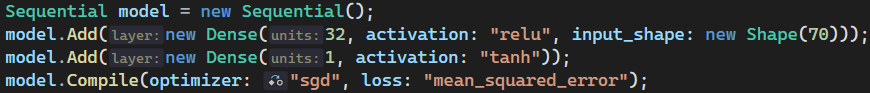
\includegraphics[width=1\textwidth]{figures/keras-model.png}
    \caption{Keras neural network}
    \label{fig:kerasModel}
\end{figure}

\subsection{Model}
\label{subsec:ch5sec1subsec2}

The implementation of the chess logic was done using several classes and enumeration types (shown in figures below). The enumeration types are $GameState$ (fig. \ref{fig:enumGameState}), $MoveType$ (fig. \ref{fig:enumMoveType}), $PieceColor$ (fig. \ref{fig:enumGameState}) and $PieceType$ (fig. \ref{fig:enumPieceType}).

\begin{figure}[h]
    \centering
    \begin{minipage}{.49\textwidth}
      \centering
      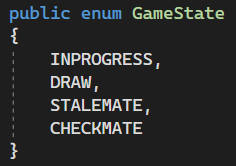
\includegraphics{figures/enum-game-state.png}
      \captionof{figure}{Game state enum}
      \label{fig:enumGameState}
    \end{minipage}
    \begin{minipage}{.49\textwidth}
      \centering
      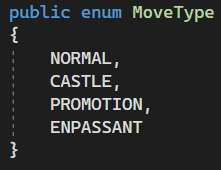
\includegraphics{figures/enum-move-type.png}
      \captionof{figure}{Move type enum}
      \label{fig:enumMoveType}
    \end{minipage}
\end{figure}

\begin{figure}[h]
    \centering
    \begin{minipage}{.49\textwidth}
      \centering
      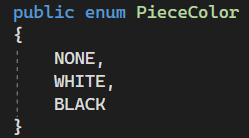
\includegraphics{figures/enum-piece-color.png}
      \captionof{figure}{Piece color enum}
      \label{fig:enumPieceColor}
    \end{minipage}
    \begin{minipage}{.49\textwidth}
      \centering
      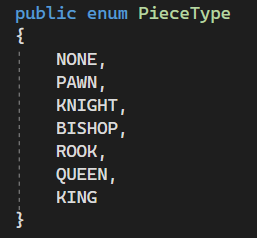
\includegraphics{figures/enum-piece-type.png}
      \captionof{figure}{Piece type enum}
      \label{fig:enumPieceType}
    \end{minipage}
\end{figure}

\subsubsection{SquareCoords}
\label{subsubsec:ch5sec1subsec2subsubsec1}

The $SquareCoords$ class encapsulates the coordinates of a square: it contains both the file number and the rank number. It has a simple constructor with the two fields as parameters, and also a constructor that receives a string parameter, checks if it is a valid square string (has two characters, first one denoting the file - a letter from $a$ to $h$, and the second one denoting the rank - a number from $1$ to $8$), and assigns the corresponding file and rank.

\subsubsection{Piece}
\label{subsubsec:ch5sec1subsec2subsubsec2}

A $Piece$ class is composed of two enumeration fields: a $PieceType$ and a $PieceColor$. I have chosen not to make a class for each piece and have it inherit a basic $Piece$ class, since the behavior of each piece differs significantly, and inheritance would complicate the implementation.

\subsubsection{Square}
\label{subsubsec:ch5sec1subsec2subsubsec3}

A $Square$ class includes the square's coordinates on the board, the piece that occupies it (which might be null if there is no piece on the square), and two boolean values, $IsAttackedByWhite$ and $IsAttackedByBlack$, which are used for the threat maps.

\subsubsection{SimpleMove}
\label{subsubsec:ch5sec1subsec2subsubsec4}

The $SimpleMove$ class contains minimal information for identifying a move: the $SquareCoords$ of the origin square, the $SquareCoords$ of the destination square, the $PieceType$ of the promotion choice (in case it is a promotion move), and an additional field with the $PieceType$ of the captured piece, used for sorting moves during the engine's search.

\subsubsection{MoveInfo}
\label{subsubsec:ch5sec1subsec2subsubsec5}

The $MoveInfo$ class contains the fields that the $SimpleMove$ class contains, plus some more fields that help during the undoing of the move: a $MoveType$ enumeration, the $Piece$ that moves, the $SquareCoords$ of the en-passant square before the move, if there was one (null otherwise), an integer denoting the previous half-move clock (how many consecutive half-moves without capturing a piece or moving a pawn were made until this move), and four boolean values denoting the previous castling rights: $PrevWhiteCanCastleKing$, $PrevWhiteCanCastleQueen$, $PrevBlackCanCastleKing$, and $PrevBlackCanCastleQueen$.

\subsubsection{Board}
\label{subsubsec:ch5sec1subsec2subsubsec6}

The $Board$ class holds the configuration of the chess board: it contains the squares of the board (which in turn contain the pieces). The squares are memorised in a two-dimensional array (fig. \ref{fig:boardClassSquares}), simplifying the process of obtaining a square on the board by file and rank.

\begin{figure}[h]
    \centering
    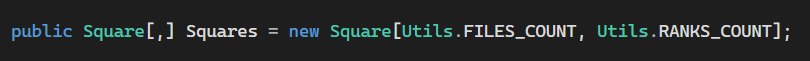
\includegraphics[width=1\textwidth]{figures/board-class-squares.png}
    \caption{The $Squares$ field of the $Board$ class}
    \label{fig:boardClassSquares}
\end{figure}

\subsubsection{Game}
\label{subsubsec:ch5sec1subsec2subsubsec7}

The $Game$ class is the largest and it contains most of the functionality needed for a chess match. It contains a $Board$ field, which denotes the coordinates of the pieces in the current game position, and other information regarding the evolution of the game:

\begin{itemize}
    \item A $PieceColor$ field denoting the player to move
    \item A $SquareCoords$ field which contains the "en-passant square", if the last move pushed a pawn two squares (the en-passant square being the square where a pawn can capture by making an en-passant move)
    \item A $GameState$ enum denoting the game's ongoing state
    \item An integer representing the number of moves since the game started
    \item An integer denoting the number of consecutive half-moves without captures or pawn moves
    \item Four boolean values denoting the castling rights
    \item A list of $MoveInfo$ objects containing the moves played in the game
    \item A list of $SimpleMove$ objects containing the legal moves in the position of the game's board
    \item A dictionary containing the positions that appeared in the game, with the key being the FEN (Forsyth-Edwards Notation) \cite{fen-desc} description of the position and the value being an integer denoting the number of times the position appeared; this is used for the threefold repetition rule
\end{itemize}

The $Game$ class has a method for setting the position from a FEN string, which contains all the necessary information for identifying a position. It is a single line of characters, made up of six fields, separated by a space.

The first field contains the piece placement, rank by rank, separated by a '/' (slash) symbol. Each piece is represented by a single character, with uppercase letters for white pieces, and lowercase letters for black pieces. A decimal digit counts consecutive empty squares on a rank. The second field specifies the player to move ('w' for white, 'b' for black). The third field indicates the castling rights - 'K' for white kingside castling, 'Q' for white queenside castling, 'k' for black kingside castling, and 'q' for black queenside castling. If no castling is possible for any side, a hyphen (-) is used. If there is a potential en passant capture available, the fourth field specifies the target square. In cases where there is no en passant target square, a hyphen (-) is used. Otherwise, the target square is represented using algebraic notation (e.g., 'e3'). The fifth field represents the halfmove clock. The sixth and last field indicates the current move number. It starts at 1 and is incremented after each black move.

Following is the FEN string representation of the starting position for a standard chess game:

\begin{figure}[h]
    \centering
    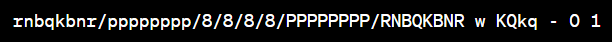
\includegraphics[width=1\textwidth]{figures/starting-position-fen.png}
    \caption{FEN string for the starting position}
    \label{fig:fenStartingPosition}
\end{figure}

The most important and complex method of the $Game$ class is $Move$. It receives as parameters two $SquareCoords$, the coordinates of the origin and destination square, and optionally a $PieceType$ parameter, which specifies the promotion piece, if it is a promotion move. Besides making the move on the board, the method checks the move to determine whether it affects any castling rights (if it is a rook move, a king move, or a rook is captured), if it changes the en passant square, checks the fifty moves rule, the threefold repetition rule, and then it updates the threat maps and the list of legal moves.

In fig. \ref{fig:depDiagram} the dependency diagram between the classes is shown.

\begin{figure}[h]
    \centering
    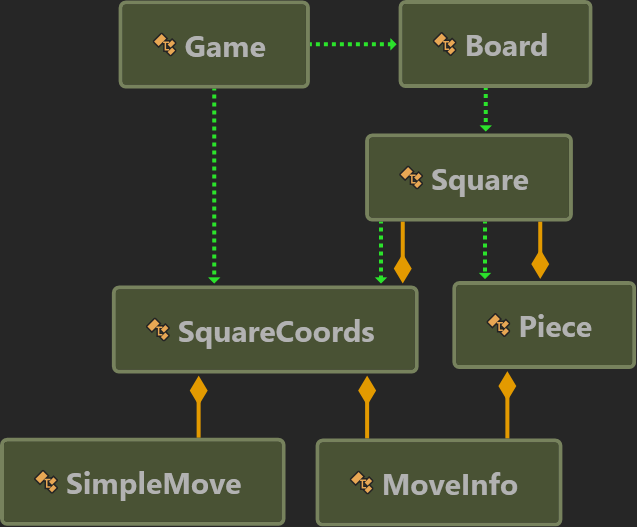
\includegraphics[width=0.6\textwidth]{figures/dependency-diagram-chess-game.png}
    \caption{Dependency diagram for the chess game project}
    \label{fig:depDiagram}
\end{figure}

\section{Chess game interface}
\label{sec:ch5sec2}
% Description of tools used in building the chess game - Unity, C\#

I created the chess interface in Unity, a game development engine that provides a visual editor and C\# scripting capabilities. I chose Unity because of its user-friendly and intuitive interface, as well as its ability to easily integrate external C\# libraries, such as the chess engine I built.

The user has the ability to select the color of the pieces he wants to play with, and also choose if he wants to control both sides or play against the engine.

On the game interface I added inputs that allow the player to change the engine parameters: the minimax depth, the usage of iterative deepening and quiescence search, and also the time limit for the iterative deepening and the maximum depth for the quiescence search (fig. \ref{fig:engineOptions}).

\begin{figure}[h]
    \centering
    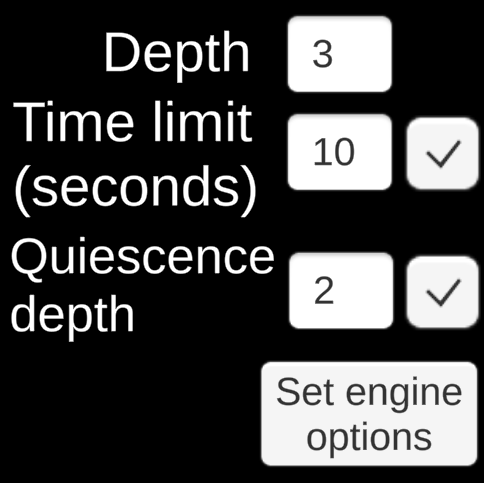
\includegraphics[width=0.4\textwidth]{figures/chess-game-engine-options.png}
    \caption{Engine options}
    \label{fig:engineOptions}
\end{figure}

The interface also contains a text box, where the user can see the current FEN and set the position from a FEN string, for the ability to quickly play against the engine from a desired position (fig. \ref{fig:fenField}).

\begin{figure}[h]
    \centering
    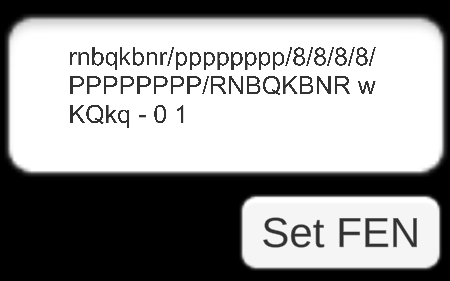
\includegraphics[width=0.4\textwidth]{figures/chess-game-fen-field.png}
    \caption{FEN field}
    \label{fig:fenField}
\end{figure}

For visibility while playing the game, when clicking a piece that has valid moves, the square of the selected piece is marked in green and the destination squares of the valid moves are highlighted in blue. Furthermore, the source square and destination square of the last played move are both marked in yellow (ex: in fig. \ref{fig:highlightedSquares}, d7 is the selected square, d6 and d5 are the destination squares of the valid moves, e2 and e3 are the source and destination squares of the previous move played).

\begin{figure}[h]
    \centering
    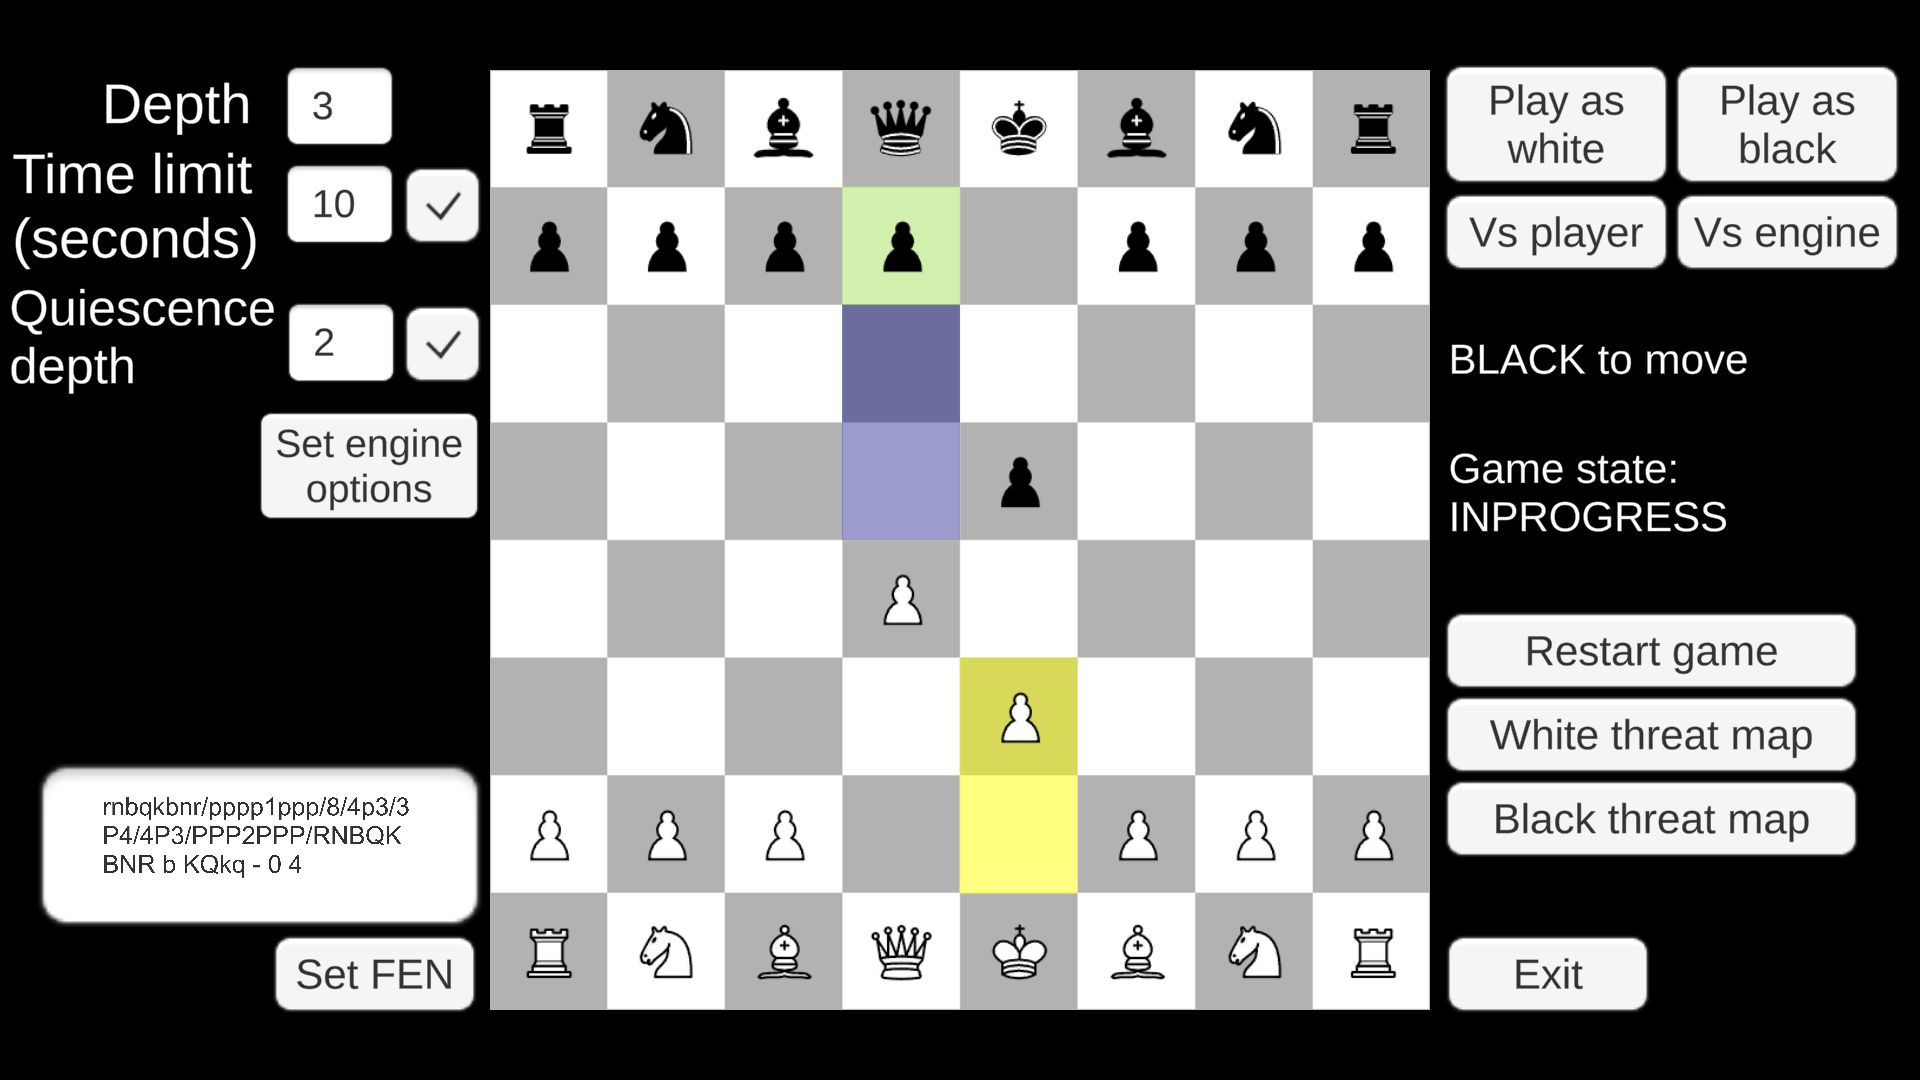
\includegraphics[width=0.95\textwidth]{figures/chess-game-squares.png}
    \caption{Highlighted squares}
    \label{fig:highlightedSquares}
\end{figure}

An additional aspect requiring consideration is providing the player with the ability to select the promotion piece upon advancing a pawn to the final rank. This has been done by displaying a box with the four valid promotion pieces (queen, rook, bishop, knight) when a player moves a pawn to the last rank (fig. \ref{fig:promotion}).

\begin{figure}[h]
    \centering
    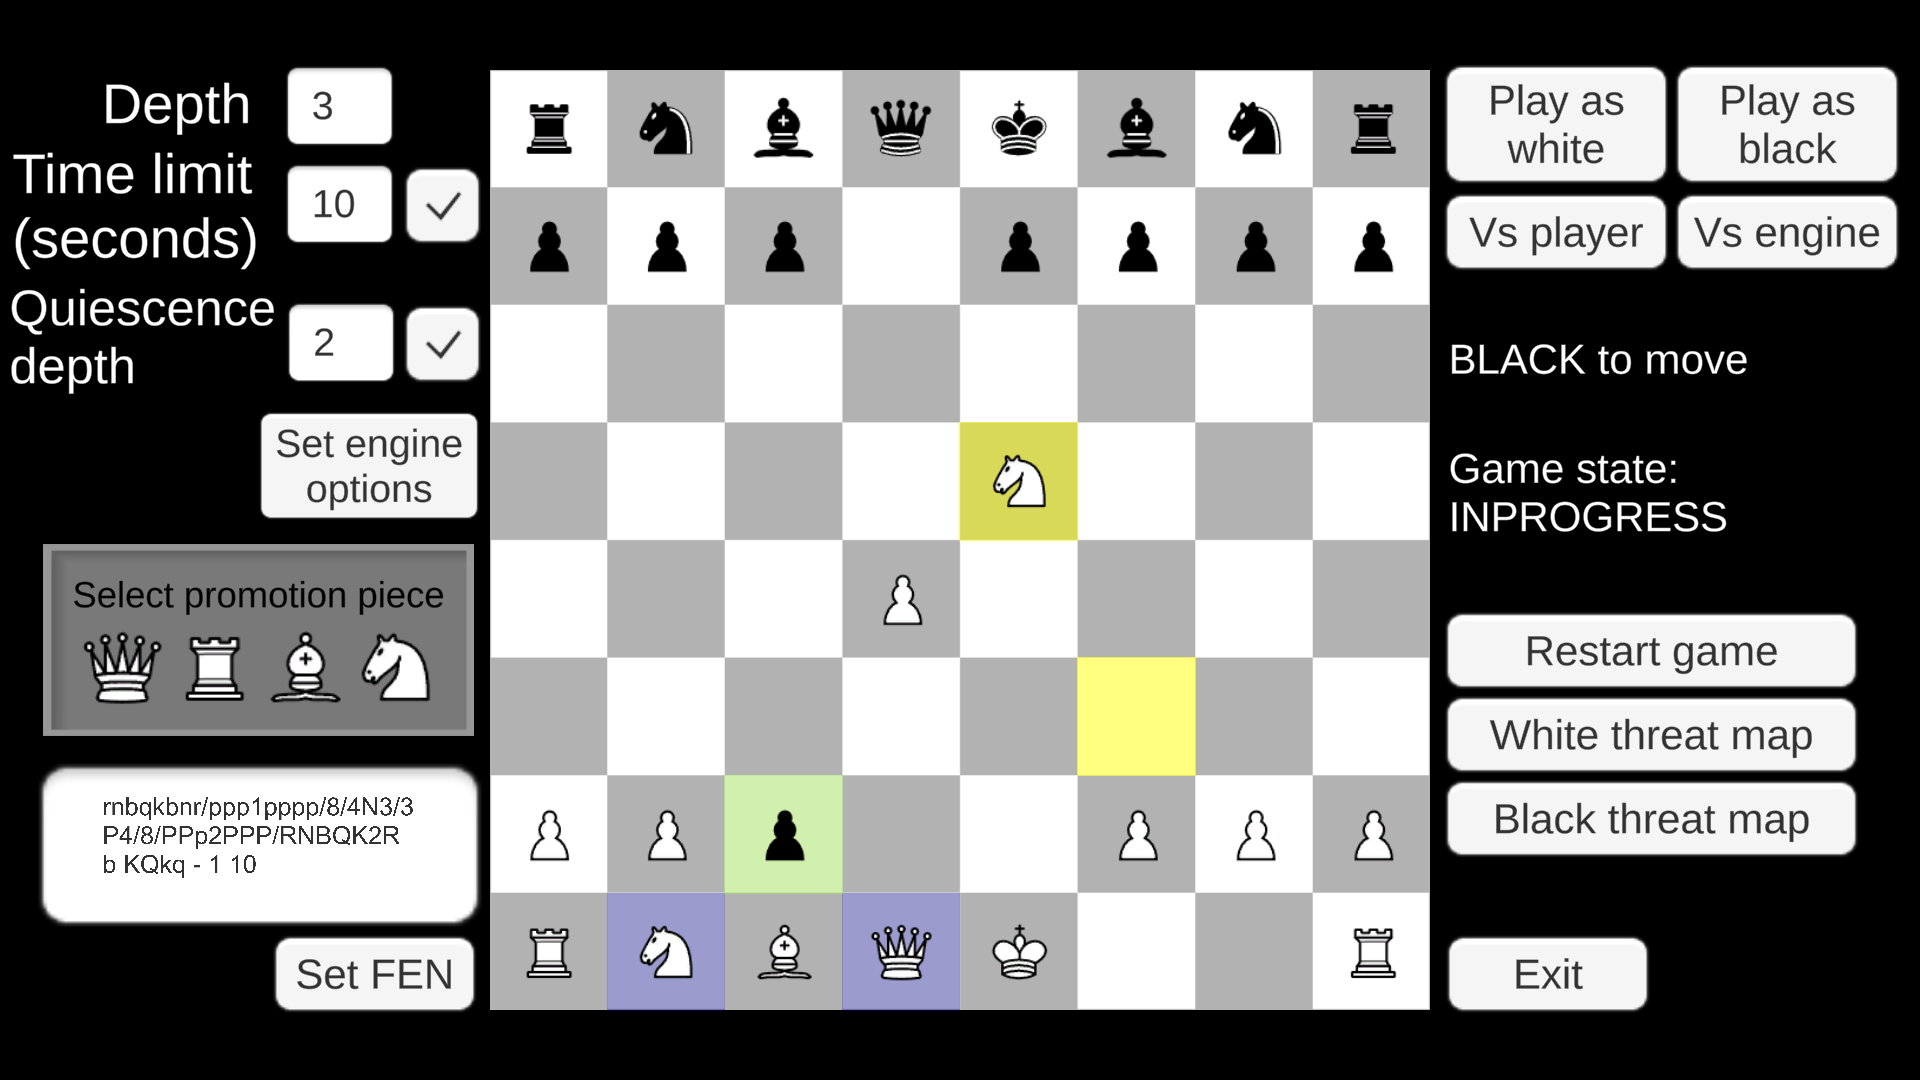
\includegraphics[width=0.9\textwidth]{figures/chess-game-promotion.png}
    \caption{Pawn promotion}
    \label{fig:promotion}
\end{figure}